\section{Hardwaredesign}
\vspace{0.5cm}
I det følgende afsnit vil de vigtigste overvejelser for designet af systemets hardware fremtræde. En mere detaljeret begrundelse for valg findes i dokumentet analyse i bilaget. Dokumentet analyse indeholder også alle de beregninger der er foretaget i forbindelse med valg af forstærkning, filtertype og subtractor.

\subsection{Forstærker}
\vspace{0.5cm}
Grundet at det signal, der udsendes gennem tryktransduceren er for småt til, at det kan analyseres og anvendes i vores system, skal signalet derfor forstærkes. Til projektet blev det givet, at signalet skulle forstærkes med en operationsforstærker af typen INA114. Denne type operationsforstærker har et variabelt gain, der afhænger af hvilken modstand, der forbindes til operationsforstærkeren.

For at vide hvor meget vi ønsker at forstærke signalet fra tryktransduceren er det vigtigt at kende til størrelsen af signalet. Mængden af forstærkning bestemmes derfor ud fra tryktransducerens følsomhed. Denne følsomhed findes i databladet for tryktransduceren. Vi udregner hvor meget vi ønsker at forstærke signalet op til:
  
\[ V_{out} =5\cdot\frac{µV}{V\cdot mmHg} \cdot 10 V \cdot 250 mmHg = 12500 µV = 12,5 mV\]

Fordi vi kender følsomheden på tryktransduceren og ved, at vi ønsker at kunne forstærke blodtrykssignaler op til 250 mmHg og har en forsyningsspænding på -5 til 5V via Analog Discovery får vi ovenstående resultat ved design af forstærkeren.

Forstærkerens gain kan udregnes med følgende formel: 
\[ G = 1+\frac{50k\Omega}{R_{G}} \]

Vi ønsker at forstærke disse 12,5 mV op til 4V. Resultatet af udregningerne blev derfor, at vi forstærker signalet fra transduceren 320 gange og bruger en modstand på 156 $\Omega$. Alle beregninger og beskrivelser findes i dokumentet analyse i bilaget.   

\subsection{Subtractor}
\vspace{0.5cm}
For at benytte alle 14-bit på AD-Converten, NI-DAQ 6009, har vi i forbindelse med designet af forstærkeren besluttet at forstærke fra 0-4V. Alle tal vi får ind fra tryktransduceren vil derfor ligge i dette område. For at få vores indgangssignal til at passe med indgangene på AD-Converten og derved udnytte alle bit er det nødvendigt at nedjustere signalet. Vi bruger derfor en subtractor af typen OP27G, som er en standard operationsforstærker, der findes i laboratoriet. Subtractoren justerer vores signal så det går fra -2V til 2V i stedet for 0-4V. Alle udregninger vedrørende subtractoren findes ligeledes i dokumentet analyse i bilaget.

\clearpage

\subsection{Anti-aliaserings filter}
\vspace{0.5 cm}
For at fjerne støj er det nødvendigt at filtrere signalet. Til systemet har vi derfor valgt at benytte et aktivt 2. ordens lavpasfilter af typen Sallen Key. Alt i alt ønskes signalet dæmpet med 90 $dB$, men fordi signalet allerede dæmpes 70 $dB$ er det kun nødvendigt at dæmpe med 20 $dB$ yderligere. Dette kan klares med et 1. ordens filter men for at være på den sikre side, har vi valgt at benytte et 2. ordens filter, der dæmper med $40 dB$ pr. dekade. Alt dokumentation omkring valg af filtertype, beregninger og begrundelse for skift at filter undervejs i projektet er beskrevet nærmere i dokumentet analyse i bilaget. Nedenfor ses opbygningen af et Sallen Key filter. Vi bruger igen en operationsforstærker af typen OP27G til at bygge filteret.

\begin{figure}[h!]
	\centering
	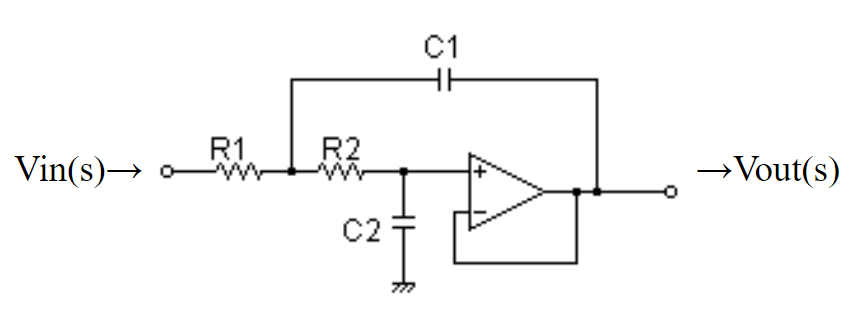
\includegraphics
	[width=0.5\linewidth]{Arkitektur_og_design/Design_hardware/SallenKey}
	\caption{Sallen Key: Aktivt 2. ordens lavpasfilter}
	\label{fig:SallenKey2}
\end{figure}

\subsection{Printplade}
\vspace{0.5 cm}
Før printpladen kan designes er det nødvendigt at opbygge systemet i Multisim. Multisim danner en simuleret version af det kredsløb, der undervejs er opbygget og testet på fumlebræt. Nedenfor vises det endelige kredsløb i Multisim, som også er brugt til at designe printpladen.

\begin{figure}[h!]
	\centering
	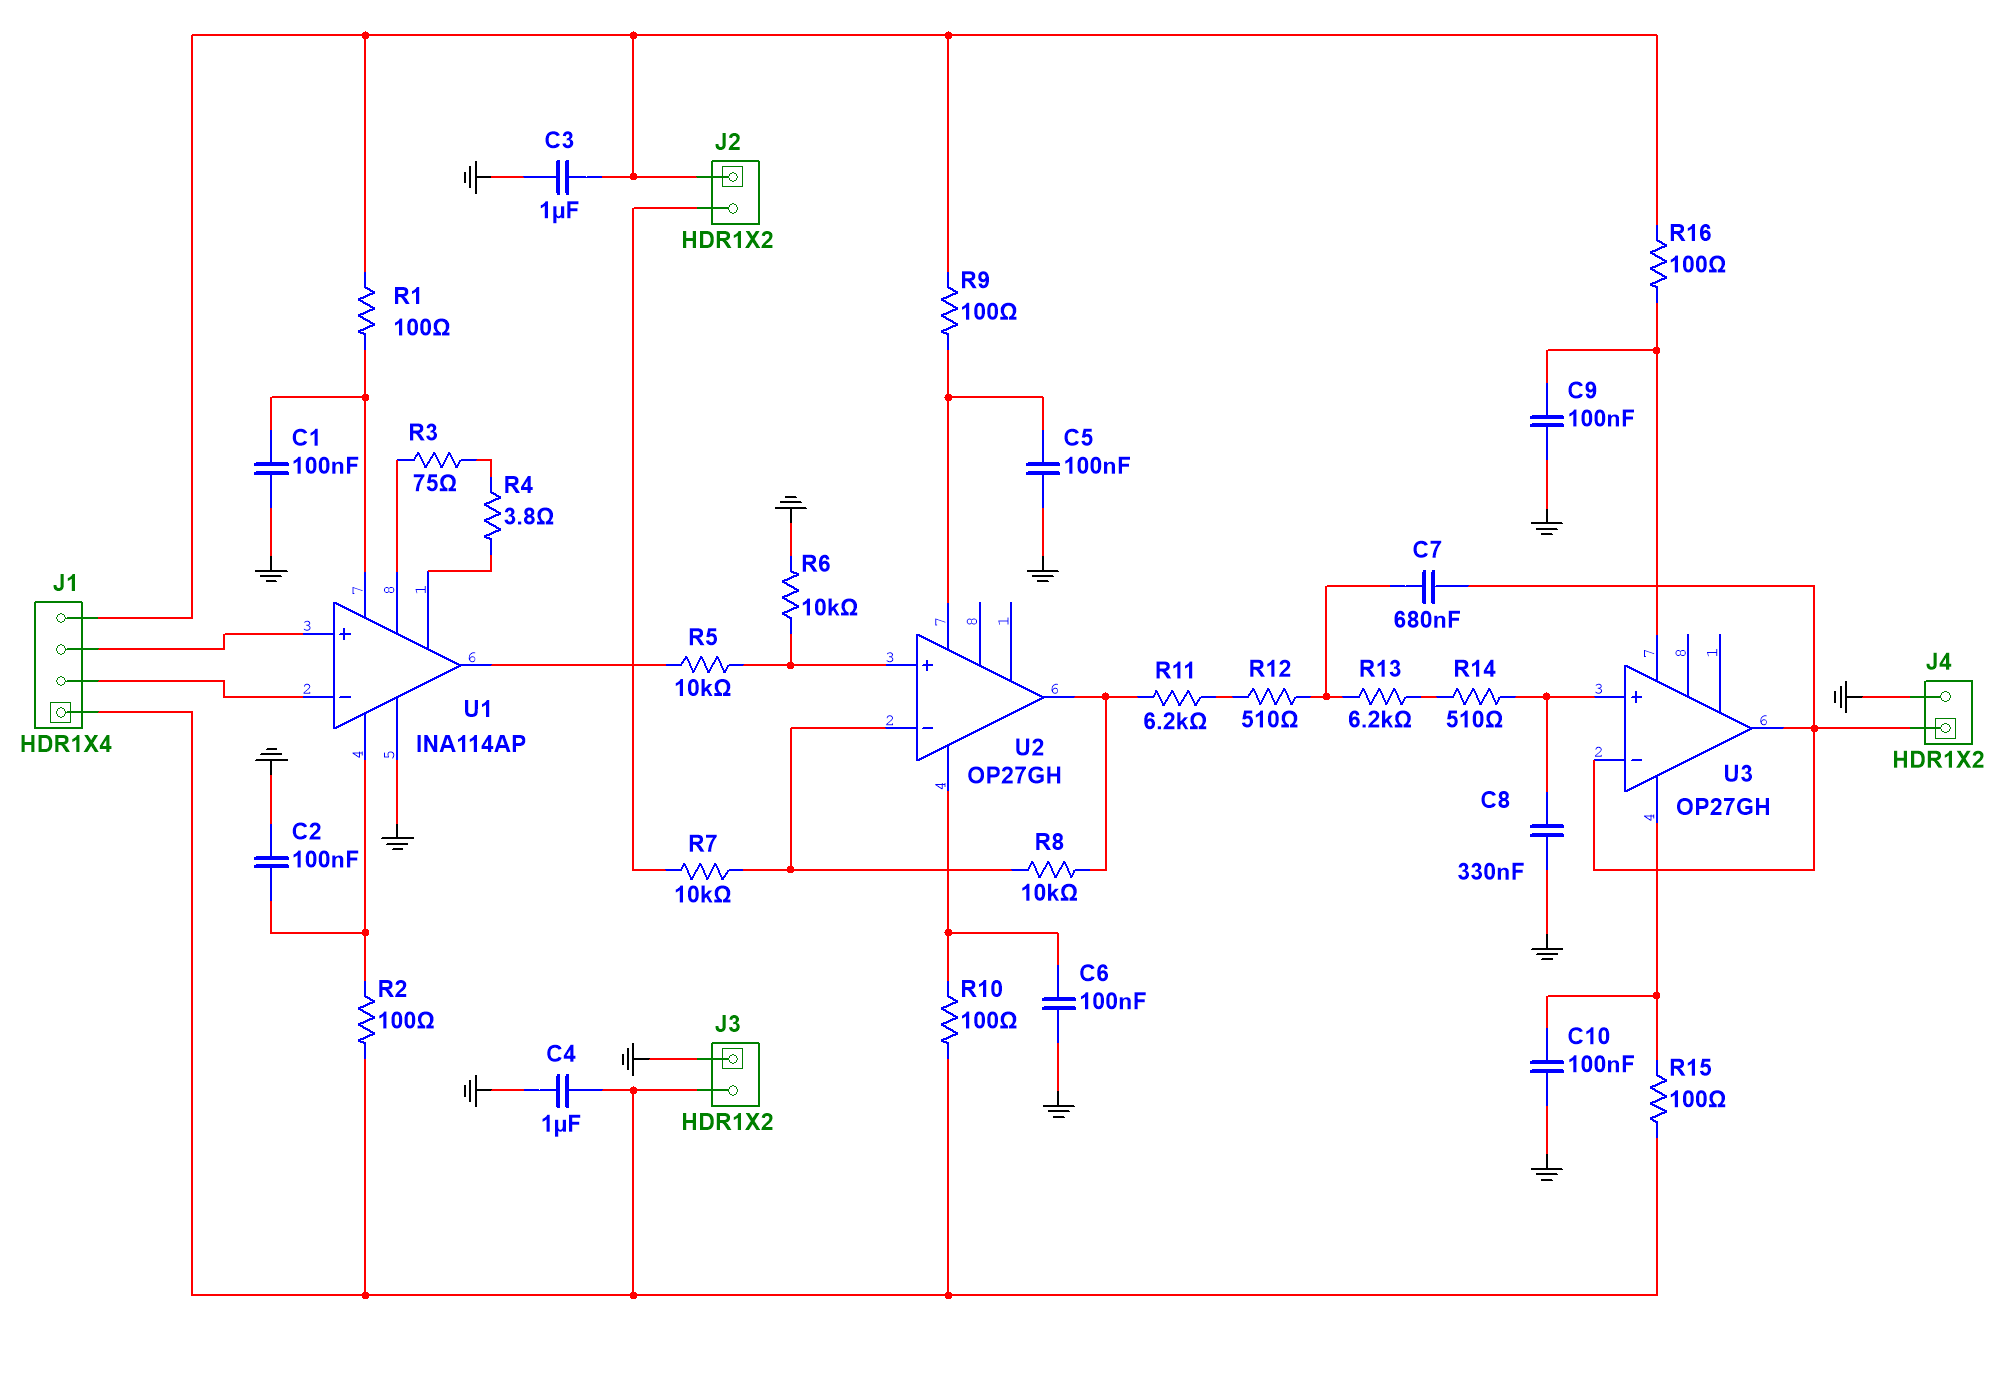
\includegraphics
	[width=0.8\linewidth]{Arkitektur_og_design/Design_hardware/Multisim}
	\caption{Kredsløbet i Multisim}
	\label{fig:Multisim2}
\end{figure}

En detaljeret beskrivelse af opbygningen af diagrammet, herunder designovervejelser, findes i dokumentet ?? i bilaget.
\clearpage